\begin{figure}[tbh]
	\centering
	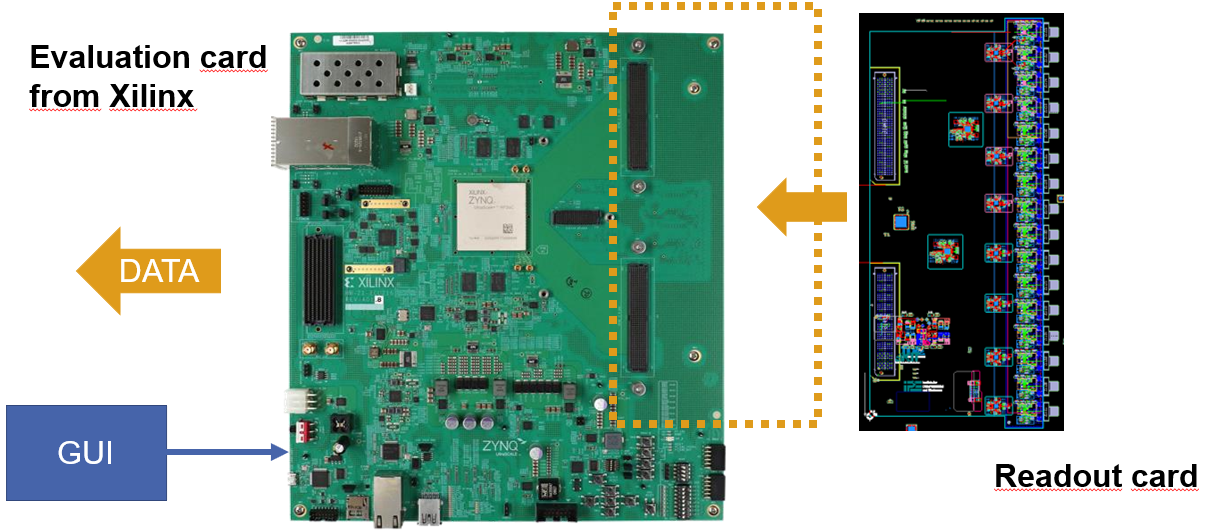
\includegraphics[width = \textwidth]{chap/04-work/img/concept_theresa}
	\caption{General concept of the new readout system}
	\label{fig:concept_theresa}
\end{figure}
\textbf{TODO:} Picture of the WHOLE system, i.e. with the optical front end + power splitter + theresa + zcu216
\section{Optical part}

\textbf{TODO} Question for serge: if they use the same setup as also described in the email or maybe some modifications?


"femtosecond Ytterbium-doped fiber laser (Orange) from MENLO GmbH. The emitted pulses have a spectral bandwidth of 50 nm, and the total
output average power is 40 mW. The repetition rate is chosen at 88 MHz, which corresponds to 1/4 th of
the RF frequency of Synchrotron SOLEIL and 104 times the electron revolution frequency."

\paragraph{Photodetector}
The detection and subtraction between the two stretched signals is performed using a amplified balanced photodetector (photoreceiver) from Discovery Semiconductors, with 20 GHz bandwidth and 2800 V/W gain (specified at 1500 nm).

\section{Front-End Card}
\textbf{TODO}


Based on the architecture of the \gls{kapture} sampling board. 
\autoref{fig:theresa_scheme} shows the general schema of the sampling system, reduced to four channels for presentation purposes.
\begin{figure}[H]
	\centering
	\includegraphics[width = \textwidth]{chap/04-work/img/theresa_scheme.tikz}
	\caption[General architecture of THERESA]{General architecture of THERESA with power splitter and \glspl{adc}. For presentation purposes only four of the sixteen channels are shown.}
	\label{fig:theresa_scheme}
\end{figure}

\section{Readout Card}
\textbf{TODO}
\section{Selection Of The Card}\label{sec:selection}
When selecting the Readout Card, following criteria need to be considered:
\begin{itemize}
	\item Integrated \glspl{adc}
	\item Number, resolution and bandwidth of \glspl{adc}
	\item Peripheral connections
	\item Flexibility/Customization
	\item Suitable connectivity for high-data-throughput
\end{itemize}

Footprint of using all discrete components is, as one can imagine, higher, than if you integrate all the parts into on \gls{ic}. Not only the footprint is a concern, but also the number of connections. ADCs with high resolution, a high number of ADCs therefore explodes the necessary amount of connections. 
\begin{figure}[tbh]
	\centering
	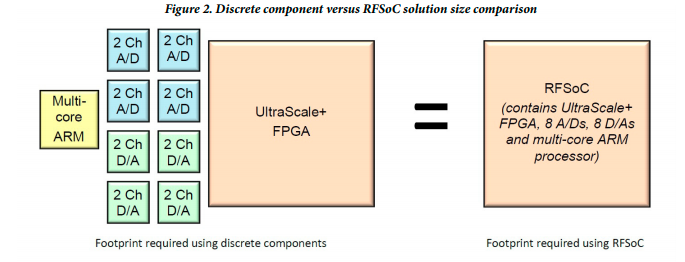
\includegraphics[width = \textwidth]{chap/04-work/img/footprint}
	\caption{Placeholder: Discrete vs IC}
	\label{fig:footprint}
\end{figure}

High number of ADCs also means 